\documentclass[a4paper, 11pt]{article}
\setlength{\topmargin}{-0.5in}
\setlength{\textheight}{9.5in}
\setlength{\oddsidemargin}{-.1in}
\setlength{\textwidth}{6.5in}
\usepackage{graphicx}
\graphicspath{ {images/} }

\title{Proposal} \author{Philip Hannant} 

\begin{document} \maketitle{} \section{Introduction \& Background}

Detecting musical time is a skill which is not only a fundamental musical skill [1] but also something that can seemingly come naturally to humans, the majority being able to analyse and reproduce discrete metrical stuctures of a piece of music [2]. Producing algorithms to replicate this nature human ability is probably first attempted by Longuet-Higgins [1], where he began to consider that rhythm as a binary tree with each node representing a note or rest. This theory developed into a system which would use a static tolerence limit on how much a the downbeats varied and enabling the perceived tempo to be adjusted accordingly [add longuet references]. Since Longuet-Higgins first work there have been a number of systems developed to perform beat tracking and temporal analysis with the majority using the ``surfboard'' method first described by schloss which observed the peaks of sound energy within a piece of music in order to discern the beat locations and temporal information [schloss]. 

This method however was not considered accurate enough to fully replicate the skill of a trained musician at beat detection, it was soon recognised that onset detection would play a fundamental part in any future beat detection algorithms. Where the an indicator of a new onset is seen as ``an increase in energy (or amplitude) within some frequency band(s)'' [4].

Need to include the different types of 

Due to the rapidly expanding research being carried out on beat detection, in 2005 the 1st annual Music Information Retrieval Evaluation eXchange (MIREX) was held. MIREX has been set up as a contest with the goal of comparing state-of-the-art algorithms and music information retrieval [MIREX website]. The topics to be evaluated were proposed by the participants and in the first year, three of the nine topics concerned beat detection (Audio Drum Detection, Audio Onset Detection and Audio Tempo Extraction).  


Needs to add history of all the work carried out on audio analysis with an emphasis on tempo detection

Beat detection and tempo analysis is a fundamental skill honed by musicians and in particularly drummers, their ability to perform at a consistent tempo determines a piece of musics rhythm. 

To date, the majority beat detection software has focused mainly on the dj industry where tempo and beat matching are popular aspects to be included in modern dj programs. There are however other sectors of the music industry would find beat detection software a useful, in particular, drummers could find it an enormously useful training tool. There are currently many systems available to a drummer, for example Roland include drum tutoring software with some of their V-Drums modules [roland ref]. These systems are however all restricted to electronic drum kits which utilise midi triggers to produce the drum sounds. The training software can therefore be easily linked to these events in order to provide live feedback on the overall tempo being played as well as which exact information on the timing of each hit on the various parts of the drum kit. 

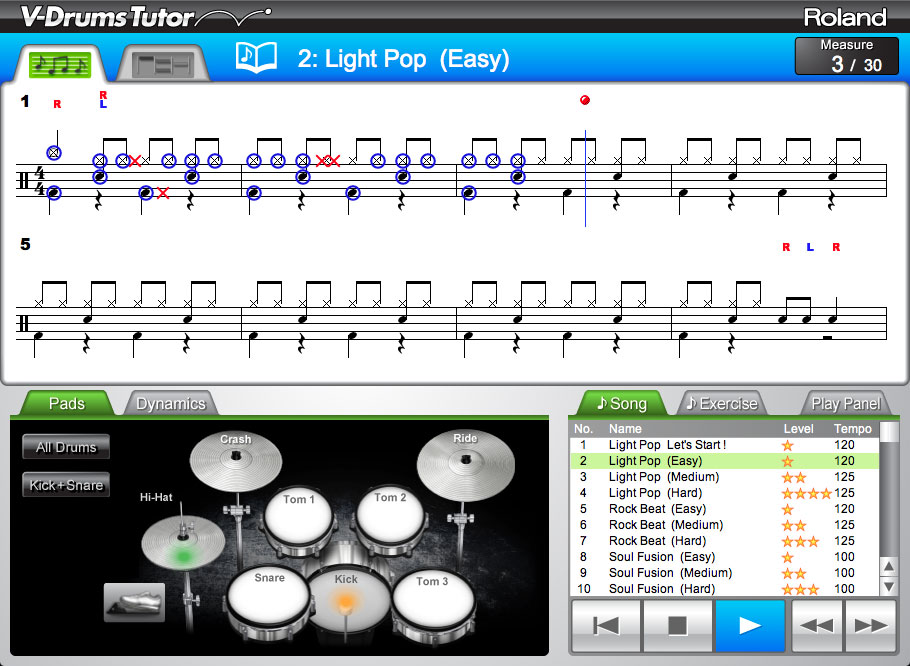
\includegraphics[scale=0.2]{dt-1_ss_main_notation_gal} 




\subsection{}

\maketitle{} \section{Aims and Objectives}
As part of my project I propose to build a real time drumbeat tempo analyser which wiill implement a variety of different wave analysis algorithms. sound energy analysis and discrete wavelet transform technologies. I will provide more details regarding the system architecture in the following sections. 

Investigate with a sole focus on drums how accurate/reliable the beatroot and discrete wavelet transform algorithms are in order to ascertain how viable a future mobile metronome and drum tempo training application would be.



\subsection{Proposed Architecture}
In order to function sufficiently the system will need to encompass the following features:

The open sourced JWave library includes a Java implementation of the Discrete Wavelet Transform (DFT) algorithm.

Beatroot has 

\begin{itemize}
\item Provide real time feedback to player on the tempo of the current drum beat.
\item 
\item Sufficent signal processing, the solution will need to process the audio in appropirate durations 
\end{itemize}




\maketitle{} 
\section{Development Plan for the Solution}

\subsection{Overview of External Libraries}



Adapt beetroot library in order to allow for efficient real time analysis

implement matlab algorithm in scala/java

develop audio capture and processing system 

\maketitle{} 
\section{Project Schedule}

\begin{table}[H]
\caption{Project Timeline} 
\centering
\begin{tabular}{ | L |c| L |}
\hline\hline 
Dates & Task & Priority\\ [0.5ex]
\hline 
Jun 13 - Jun 19 & Integrate APIs and external libraries & MUST
\end{tabular}
\label{stages} 
\end{table}

\maketitle{} 
\section{References}
http://www.roland.co.uk/blog/exploring-roland-dt-1-v-drums-tutor-software/


\end{document}
